\documentclass{article}
\usepackage{hyperref} 
\usepackage[utf8x]{inputenc}
\usepackage[spanish]{babel} 
\usepackage{libertine}
\usepackage[T1]{fontenc}

\setcounter{tocdepth}{2}

% Necesitamos los paquetes graphicx, caption y subcaption
\usepackage{graphicx}
\usepackage{wrapfig}
\usepackage{caption}
\usepackage{subcaption}
\usepackage{float}
\usepackage{multirow}
\usepackage[spanish]{babel}

\usepackage{enumitem}

\usepackage{vmargin}

\setpapersize{A4}
\setmargins{2.5cm}      % margen izquierdo
{1.5cm}                 % margen superior
{16.5cm}                % anchura del texto
{23.42cm}               % altura del texto
{10pt}                  % altura de los encabezados
{1cm}                   % espacio entre el texto y los encabezados
{0pt}                   % altura del pie de página
{2cm}

\title{DSED PROYECTO FINAL}

\author{Carlos Gómez Rodríguez y Alejandro Ramos Martín}

%\date{15 de Diciembre, 2019}

\begin{document}

\maketitle

\tableofcontents

\newpage

\section{Bloque 1: Interfaz de audio}

\subsection{Tarea 1.1:}
\paragraph{Diseña un circuito que sea capaz de generar las señales especificadas. Dibuja el esquemático correspondiente a tu diseño en el espacio inferior.}

\subsection{Tarea 1.2:}
Implementa tu diseño en VHDL.

\subsection{Tarea 1.3:}
Genera un testbench que verifique la funcionalidad de tu diseño.
\newpage
\subsection{Tarea 1.4:}
Realiza el diagrama ASMD que describa la misma funcionalidad que el pseudo-código anterior.

\begin{figure}[H]
\centering
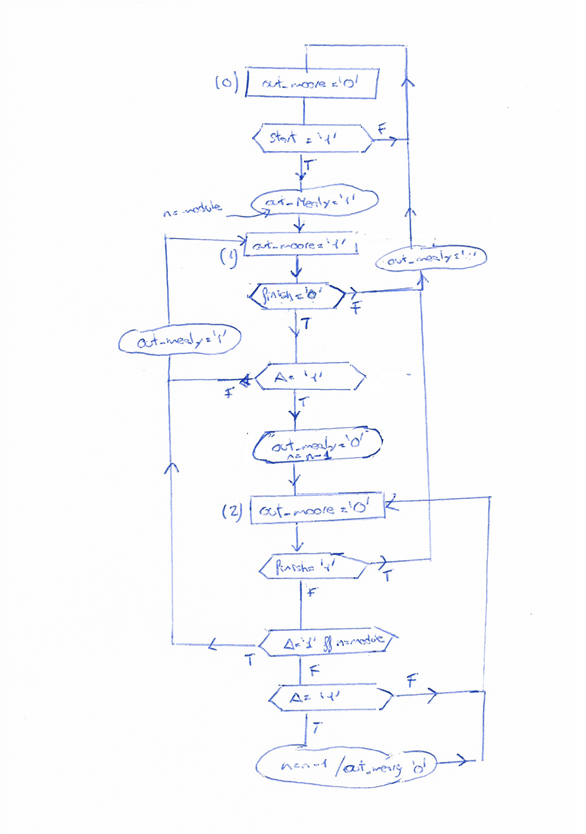
\includegraphics[width=0.9\linewidth]{images/1_4.png}
\end{figure}

\subsection{Tarea 1.5:}
Implementa el diagrama anterior en un fichero VHDL.

\subsection{Tarea 1.6:}
Realiza un testbench que tenga la señal micro data fija a '1' para comprobar que las transiciones de estados, la selección de los datos de salida y la activación de sample{\_}out{\_}ready se produce correctamente.

\subsection{Tarea 1.7:}
Realiza un testbench que introduzca una se˜nal pseudo-aleatoria en micro data y comprueba que la digitalización se realiza correctamente.

\subsection{Tarea 1.8:}
Modifica el diseño propuesto en el libro del Dr. Chu para que sea compatible con las especificaciones de nuestro sistema. Es decir, que el contador cuente de 0 a 299 e incluya reset y enable y que el circuito produzca la salida sample request en el momento apropiado y con la duración apropiada. Dibuja el esquem´atico de tu diseño en la parte inferior.

\subsection{Tarea 1.9:}
Implementa el esquemático anterior en un fichero VHDL.

\subsection{Tarea 1.10:}
Realiza un testbench que verifique el funcionamiento de la interfaz de la salida de audio.

\subsection{Tarea 1.11:}
Dibuja el esquemático a nivel bloque de la interfaz de audio completa. Ten en cuenta que record enable y play enable especifican cuándo están activas las interfaces del micrófono y de la salida de audio, respectivamente. Del mismo modo, tienes que asignar un `1' tanto a micro LR, como a jack{\_}sd.

\subsection{Tarea 1.12:}
Implementa en VHDL la interfaz de audio completa. Para ello utiliza un estilo de código estructural que instancie cada uno de los tres bloques desarrollados anteriormente.

\subsection{Tarea 1.13:}
Diseña un testbench que verifique la funcionalidad de la interfaz de audio completa.

\subsection{Tarea 1.14:}

Implementa en VHDL el controlador. Utiliza estilo estructural. Necesitas emplear el asistente arquitectural de Vivado para generar el reloj de 12 MHz a partir del rejol de 100 MHz.

\subsection{Tarea 1.15:}

Diseña un testbench que verifique la funcionalidad del controlador. Puedes utilizar los estímulos empleados en testbenches anteriores.

\subsection{Tarea 1.16:}

Escribe el fichero de restricciones .xdc. Sintetiza y realiza la implementaci´on física del diseño. Genera el fichero .bit y programa la FPGA. Comprueba el funcionamiento correcto conectando unos auriculares a la salida de audio de la placa. Si la salida de audio es muy ruidosa, puedes jugar con el valor de micro LR y ponerlo a ’0’ en lugar de a '1'.
Guarda en un fichero de texto todos los mensajes de warning que hayan aparecido en el proceso anterior.
Avisa al profesor para comprobar el funcionamiento.

\section{Bloque 2: Filtro FIR}

\subsection{Tarea 2.1:}
¿Cuál es el rango de un número de 8 bits en punto fijo <1,7> en complemento a dos?
¿Cuál es su precisión?
\begin{figure}[H]
\centering
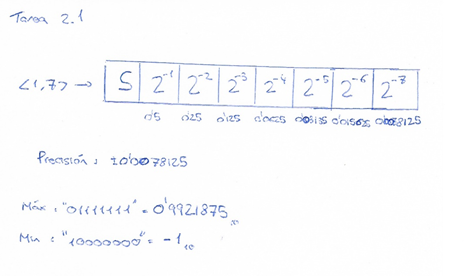
\includegraphics[width=1\linewidth]{images/2_1.png}
\end{figure}

\newpage
\subsection{Tarea 2.2:}
Realiza sobre papel la implementaci´on de un filtro FIR de 5 etapas con la siguiente asignación: Dos medios multiplicadores y un sumador. Realiza todos los pasos descritos en la sección 6.4.

\paragraph{ Planificación temporal}



\paragraph{Vinculación, análisis de tiempo de vida de variables y asignación de registros:}

\begin{figure}[H]
\centering
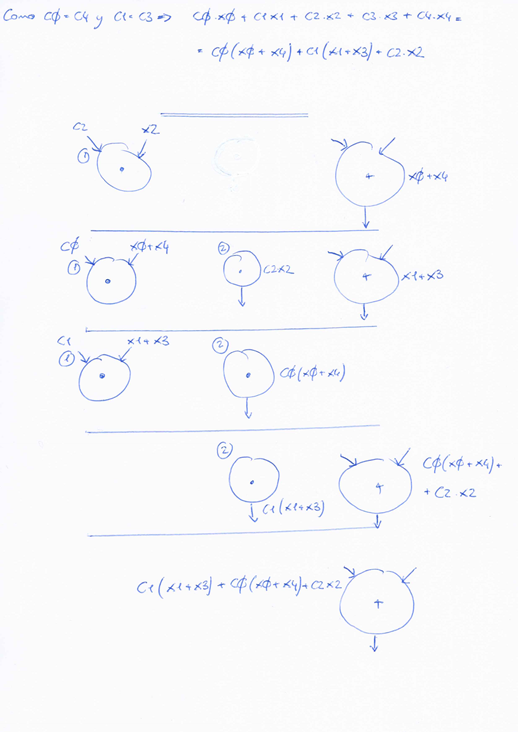
\includegraphics[width=0.85\linewidth]{images/2_2_1.png}
\end{figure}

\paragraph{Análisis de conexiones para la extracción de multiplexores:}


\paragraph{Cronograma:}

\paragraph{Implementación:}

\subsection{Tarea 2.3:}

Realiza un análisis de cuantificación de las señales, de manera que especifiques cuántos bits vas a emplear en cada señal y en qué posición va a estar el punto decimal. Emplea la notación y las metodologías presentadas en clase.

\subsection{Tarea 2.4:}

Escribe modelos VHDL para todos los componentes que se emplean en tu ruta de datos. Los operadores aritméticos (suma y multiplicación) no necesitan describirse en un estilo estructural. Para conseguir el medio multiplicador, añade un registro extra a la salida de un multiplicador completo, de esta forma se comportará como un multiplicador perfectamente segmentado. La herramienta de síntesis se encargará de mover este registro al interior del multiplicador de manera óptima. Comprueba el funcionamiento correcto de tus componentes creando los correspondientes testbenches.

\subsection{Tarea 2.5:}
Escribe un modelo estructural de la ruta de datos completa en VHDL. Crea un testbench para la ruta de datos.

\subsection{Tarea 2.6:}

Dibuja el diagrama de estados que describe el controlador de tu filtro FIR. Sigue la metodología de implementación de máquinas de estados finitos vista en clase.

\subsection{Tarea 2.7:}

Escribe el código VHDL correspondiente a tu controlador.

\subsection{Tarea 2.8:}

Escribe el código VHDL estructural correspondiente a tu filtro completo.

\subsection{Tarea 2.9:}

Escribe el código VHDL correspondiente a un testbench que introduzca un único impulso a la entrada de valor +0.5. ¿Qué secuencia esperas en Sample{\_}Out si en Sample{\_}In la secuencia es (0, 0, 0, 0, X, 0, 0, 0, 0)? Considera que X es el mayor/menor número positivo/negativo (cuatro casos) que se puede representar. Ten en cuenta la cuantificación
de tus señales. Asegúrate de que tu diseño proporciona los valores esperados.

\subsection{Tarea 2.10:}

Escribe el código VHDL correspondiente a un testbench que introduzca en la entrada
la siguiente secuencia (0, 0.5, 0, 0.125, 0, 0, 0, 0, ...). ¿Qué secuencia esperas en Sample{\_}Out para esta secuencia de entrada? Asegúrate de que tu diseño proporciona los valores esperados.

\subsection{Tarea 2.11:}
Escribe el código VHDL correspondiente a un testbench que lea las muestras de un fichero y escriba los resultados en otro.
Llama al fichero que contiene los datos de entrada “sample{\_}in.dat”; llama al fichero de salida “sample{\_}out.dat”.
Rellena el fichero de entrada con una secuencia que introduzca un único impulso.
Cada línea del fichero se corresponde con un dato.

\subsection{Tarea 2.12:}

Utiliza el fichero “haha.wav” en Matlab para crear un fichero de entrada para tu testbench. En el ap´endice 2 se detallan las secuencias que tienes que emplear en Matlab para:
Cargar un fichero de audio en Matlab y crear otro fichero con el formato necesario para tu testbench.
Utilizar la función filter de Matlab para obtener la respuesta de un filtro FIR con precisión real.
Cargar y escuchar la salida que ha producido tu testbench en Matlab.

\subsection{Tarea 2.13:}
Emplea tu testbench para procesar el fichero de entrada que te ha proporcionado
Matlab. Escribe los datos filtrados en el fichero “sample{\_}out.dat”, que importarás posteriormente en Matlab.

\subsection{Tarea 2.14:}
Importa tu fichero ``sample{\_}out.dat'' en Matlab. Compara los resultados del testbench con los valores con precisión real proporcionados por la función filter de Matlab. Haz un gráfico del error de tus resultados (resta tus resultados de los datos con precisión real).
Utiliza la función sound de Matlab para escuchar la forma de onda original. Compárala después con tu sonido filtrado y observa si hay alguna diferencia entre el filtro con precisión real y tu filtro.

\section{Bloque 3: Controlador y Memoria}

\subsection{Tarea 3.1:}
Tarea 3.1:
Crea un testbench que trabaje a la frecuencia del sistema para comprobar y entender el funcionamiento de la memoria encapsulada. Anota a continuación la función de cada
puerto y la temporizaci´on de la memoria (un peque˜no cronograma que incluya una escritura y una lectura).

\subsection{Tarea 3.2:}

Determina cuánto tiempo de grabación va a poder estar almacenado en la memoria.

\subsection{Tarea 3.3:}
Determina qué operación es necesaria para hacer la transformación de las muestras de binaria a complemento a dos y de complemento a dos a binaria.

\subsection{Tarea 3.4:}
A˜nade a continuación todas las hojas necesarias para describir tu dise˜no y la planificación para llevarlo a cabo. Puedes incluir diagramas esquemáticos, cronogramas explicativos, un plan de pruebas, una planificación temporal y todo lo que consideres necesario para explicar las decisiones que has tomado.
Avisa al profesor antes de comenzar con el dise˜no para obtener el visto bueno.

\subsection{Tarea 3.5:}
Avisa al profesor cuando tengas todas las especificaciones mínimas del sistema global cubiertas.

\subsection{Tarea 3.6:
}
Sube al Moodle un fichero .vhd con todas las fuentes de tu proyecto.

\subsection{Tarea 3.7 (Opcional):}
A˜nade a continuación todas las hojas necesarias para describir las mejoras que hayas implementado.

\end{document}
